\section{Reaching}
\label{sec:reaching}

In this section, we describe the two approaches we followed to solve
the reaching task on our robot.The first method 
uses the forward mapping between the arm joint space and the three 
dimensional position of the hand represented in the head reference 
frame $\begin{bmatrix} \theta_y & \theta_p & \alpha_v^d\end{bmatrix}^\top 
\in \mathbb R^3$. 
The second method uses a visual servoing technique to control the 
speed of the arm to minimize the position of the hand in the 
image plane with respect to a desired target (usually the fixated object).

\subsection{Open Loop Reaching}
%
Suppose the robot is tracking a target using the control strategy described in 
Section \ref{Sec:TrackerController}. In the assumption of perfect 
tracking (the visual error is zero), the three dimensional spatial position 
of the target with respect to the robot, denoted $\tilde {\mathbf x}_{target} 
\in \mathbb R^3$, 
is a function of the head configuration $\mathbf q_{head} =
\begin{bmatrix} \theta_y & \theta_p & \theta_r & \alpha_v^d & \alpha_v^c & \alpha_t^c \end{bmatrix}^\top \in \mathbb R^6$.
However, the representation of the target position, 
$\tilde {\mathbf x}_{target}$, in terms of the full head configuration, 
$\mathbf q_{head}$, is clearly redundant.
Specifically, the same target position can be represented by different 
head configurations. To obtain a one to one mapping between the target 
position and the head configuration we have to analyze the 
{\tt tracker controller}. The latter maintains $\theta_r$ stationary 
($\theta_r^d = 0$) and poses additional constraints on the head joints. 
In particular we know from section \ref{Sec:TrackerController} that the 
controller minimizes $\alpha_t^c$ and $\alpha^c_v$ (see equation 
(\ref{Eq:HeadEyeControl})) so that they asymptotically
converge to zero ($\alpha_t^c \rightarrow 0$ and 
$\alpha_v^c \rightarrow 0$). Ideally, after 
fixation is achieved, we have:
%
\begin{eqnarray}
{\mathbf q}_{head}=
\begin{bmatrix} \theta_y & \theta_p & 0 & \alpha_v^d & 0 & 0 \end{bmatrix}^\top \in \mathbb R^6.
\end{eqnarray}
%
Since there exists a one to one mapping between the three dimensional 
position of the target 
$\tilde {\mathbf x}_{target}$ and the three non-zero variables 
$\theta_y$, $\theta_p$ and $\alpha_v^d$, we can define:
%
\begin{eqnarray}
\mathbf x_{target}=
\begin{bmatrix} \theta_y & \theta_p & \alpha_v^d\end{bmatrix}^\top \in \mathbb R^3.
\end{eqnarray}
%
This new variable $\mathbf x_{target} \in \mathbb R^3$ uniquely codes the 
spatial position of the target in a way that resembles a three dimensional 
polar representation. In particular $\theta_y$ and $\theta_p$ code 
respectively \emph{azimuth} and \emph{elevation}, while \emph{distance} is 
substituted with $\alpha_v$ (the \emph{vergence} angle). 

If the robot tracks the hand, the same subset of the head joint space 
can be used to code the spatial location of the hand:
%
\begin{eqnarray*}
\xhand=
\begin{bmatrix} \theta_y & \theta_p & \alpha_v^d\end{bmatrix}^\top \in \mathbb R^3.
\end{eqnarray*}
%
Under these assumtions, the \emph{forward mapping} 
$f_{arm} : \mathbb R^3 \longrightarrow \mathbb R^4$
relates the arm configuration $\qarm$ with the position of the hand 
$\xhand$:
%
\begin{equation} 
\label{Eq:forward}
\mathbf x_{hand}=f_{arm}(\mathbf q_{arm}), \qquad f_{arm} : \mathbb R^3 \longrightarrow \mathbb R^4.\end{equation}
%
It is easy to train a neural network to  approximate the arm forward mapping 
(Eq. \ref{Eq:forward}): 
%
\begin{equation} 
\label{Eq:forward2}
\mathbf x_{hand}=\hat{f}_{arm}(\mathbf q_{arm}), \qquad \hat{f}_{arm} : \mathbb R^3 \longrightarrow \mathbb R^4.\end{equation}
%
Suppose now that the robot is fixating a target and that we want to control 
the robot to reach for it. Formally the problem can be formulated 
as determining the value of $\qarm$ which solves the 
following minimization:
%
\begin{equation} 
\label{Eq:reaching1}
  \displaystyle\min_{\qarm} \left(J\right)=\displaystyle\min_{\qarm}
  \left\|\mathbf x_{hand} - \mathbf x_{target}\right\|^2,
\end{equation}
%
where $\mathbf x_{target}$ is measured from the encoders of the head, while 
$\mathbf x_{hand}$ is computed from $\qarm$ through Eq. (\ref{Eq:forward2}).
Given the redundancy of the arm kinematics the minimization 
(\ref{Eq:reaching1}) has infinite solutions. We constrained the problem by 
forcing one of the joints, for example joint number 2, to remain as close 
as possible to a predefined value $q_{20}$:
%
\begin{equation} 
\label{Eq:reaching2}
  \displaystyle\min_{\qarm}\left(J_c\right)=\displaystyle\min_{\qarm}
  \left[
  \left\|\mathbf x_{hand} - \mathbf x_{target}\right\|^2 + \left(q_{arm,2}-q_{20}\right)^2
  \right].
\end{equation}

The optimization of (\ref{Eq:reaching2}) can be performed numerically with 
different tools. Discussing the different properties of these numerical 
tools falls outside the scope of this paper. In our implementation, we used 
the downhill simplex method \cite{ne:Computer:65} as implemented in 
\cite{mo:Press:90}.

\subsection{Learning the open loop reaching}
\label{sec:learning-open-loop}
%
To learn the forward map of Eq. (\ref{Eq:forward}) we programmed 
the robot to perform random movements with the arm (chosen to uniformly sample 
a predefined region in the robot workspace). During this ``exploratory'' 
phase the robot tracked the hand, and collected samples of the form:
%
\begin{center}
\begin{math}
  \left(\begin{array}{cc}
    \qarm^i , \xhand^i\end{array}\right)_{i \in 0,1\dots}
\end{math}
\end{center}
%
A neural network was then trained to learn the relation:
%
\begin{equation} 
  \xhand=\hat{f}_{arm}\left(\qarm \right),
\end{equation}
%
which approximates Eq. (\ref{Eq:forward}).

In the experiment reported in this paper we collected a data set of 
about 2890 samples that we devided in a training set (2168 samples) and 
a test set (725 samples). The neural network we employed was the 
Receptive Field Weighted Regression model proposed 
by \cite{schaal98Constructive}. This network implements an online learning
method, meaning that a learning step is performed every time a new 
sample is shown to the network. All samples in the training set were shown
to the network in a random order. After each training step the 
performance of the network was validated on the whole test set, by computing
the mean squared error between each sample in the test set and the 
corresponding network output. The plot in figure (\ref{fig:reaching-error})
shows the trend of the error on the test set during learning. At the end of
the training the network reached the performance of $\emph{mse}=5.7$ 
with $\emph{std}=10.4$.

In the experiment reported in this paper the network was trained offline. 
This was to simplify the analysis of the results and perform cross-validation 
on a predefined test set. However, the learning algorithm we used was purely 
incremental (each sample was shown to the network only once and immediatly 
discarded), so in this regard it will be straightforward to have an 
online implementation of the same mechanism.

\begin{figure}[tbp]
\label{fig:reaching-error}
\centerline{
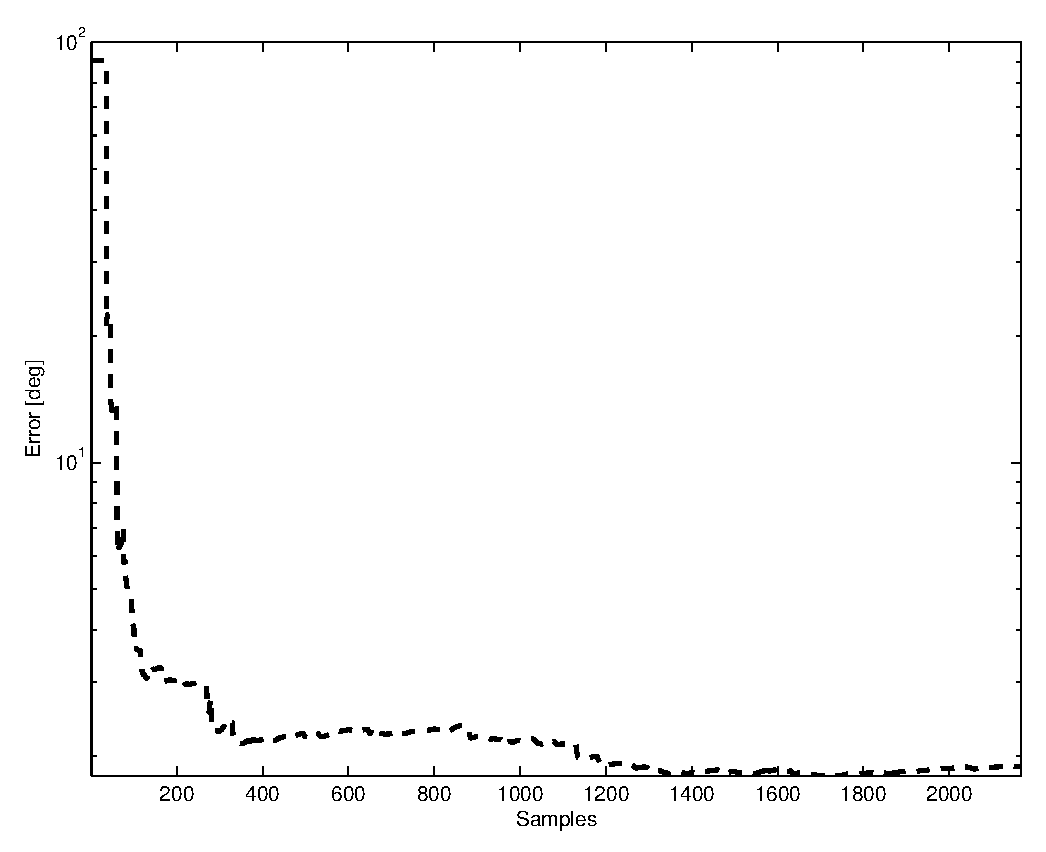
\includegraphics[width=4.0in, angle=0 ]{./Figure/reachingError1.eps}
} \caption{Learning of the arm forward function. The plot reports the \emph 
on the test set during learning. See text.}
\end{figure}

\subsection{Closed Loop Reaching} \label{Eq:ClosedLoop}
%
If the robot can visually measure the distance
between the hand and the target, reaching can also be solved
visually, by implementing a closed loop control.

We know that the Jacobian matrix relates movement of the arm 
$\deltaqarm$ in the joint space with displacement of the hand 
\begin{math}\deltauhand=
\left[ \begin{array}{ccc}
  \delta u_r & \delta v_r & \delta u_{lm}
\end{array} \right]^T\end{math} 
in the image plane, formally:
%
\begin{equation} 
\label{eq:jacobian1}
  \deltauhand=
  \tilde{\mathbf J}\left(\mathbf q_{arm}, \mathbf q_{head}\right)
  \deltaqarm,
\end{equation}
%
where $\tilde{\jacobian} \in \mathbb R^{3 \times 4}$ depends on 
both the configuration of the arm and the head. Due to the 
additional constrained posed by the head tracker, we showed
that only a subset of $\qhead$, $\xtarget$, is 
sufficient to uniquely identify the position of the head, so we 
can rewrite equation (\ref{eq:jacobian1}) as:
%
\begin{equation}
\label{eq:jacobian2}
  \deltauhand=
  \tilde{\jacobian}\left(\qarm, \xtarget\right)
  \deltaqarm, \qquad \tilde{\jacobian} \in \mathbb R^{3,4}.
\end{equation}
%

Moreover, from equation (\ref{Eq:forward}) it is clear that 
$\qarm$ and $\xtarget$ are redundant and that only $\qarm$ is 
sufficient to uniquely identify the position of the head. Eq.
(\ref{eq:jacobian2}) can be further simplified to:
%
\begin{equation} 
\label{eq:jacobian3}
  \deltauhand=
  \jacobian \left(\qarm\right)
  \deltaqarm,\qquad \jacobian \in \mathbb R^{3,4}
\end{equation}
%
in which $\jacobian$ depend only on the arm joint configuration $\qarm$.

Suppose now the robot has to reach for an object, whose visual position is 
represented by $\utarget$. To solve this problem 
the controller of the arm needs to compute the arm command which minimizes 
the error:
%
\begin{equation}
  e=\left||\uhand-\utarget\right||^2.
\end{equation}
%
When the head tracker has achieved convergence on the object, 
$\utarget \approx 0 $ and $e$ $\approx \left||\uhand\right||^2$.
Due to the redundancy of the arm, the minimization of $e$ can have
infinite solutions. Among them, the minimum norm solution corresponds
to the one which produces the minimum joint speeds, that is:
%
\begin{equation}
\mathbf{\dot q}_{arm}=-k \cdot \jacobian^\# \uhand, 
\qquad \jacobian^\# \in \mathbb R^{4,3},
\end{equation}
%
where $\jacobian^\#$ is pseudo-inverse of $\jacobian$).

\subsection{Learning the Arm Jacobian}
%
In the previous section we used the Jacobian of the manipulator
$\jacobian$ (actually its pseudo-inverse $\jacobian^\#$) to 
control the arm to reach for a visually identified object. In 
this section we describe a procedure by which the robot can 
autonomously acquire $\jacobian$ and $\jacobian^\#$.

As described in Section \ref{sec:learning-open-loop}, the robot 
moves the arm randomly, while maintainining gaze on the hand. At 
the end of each movement $j$ the arm is in a configuration 
$\qarm^j$,  while the eyes are fixating the hand 
($\uhand \approx 0$) with the gaze centered within the neck 
(the head tracker has been reached convergence). Each 
arm configuration corresponds to a different value of 
$\jacobian_j=\jacobian\left(\qarm^j\right)$. 
Now the robot inhibits the head tracker and performs a sequence $m$
of small arm movements $\deltaqarm^k$ which perturb 
$\uhand$ of small amounts $\deltauhand^k$:
%
\begin{center}
\begin{math}
  \left(\begin{array}{cc}
    \deltauhand^k , 
	\deltaqarm^k \end{array}
  \right)_{k \in 0,1\dots,m}
\end{math}
\end{center}
%
All $m$ perturbations $\deltauhand^k$ and 
$\deltaqarm^k$ are linearly realated thourgh $\jacobian_i$ 
as described in Eq. (\ref{eq:jacobian2}). From these $m$ 
observations we can derive a least squares estimation of $\jacobian_j$ from 
which, in turn, we can compute the pseudo-inverse $\jacobian_j^\#$. 

Re-iterating this procedure leads to the collection of a series of examples:
%
\begin{center}
\begin{math}
  \left(\begin{array}{cc}
    \qarm^j , \jacobian_j^\# \end{array}\right)_{j \in 0,1\dots}
\end{math}
\end{center}
%
An approximation $\hat{\jacobian}^\#$ of $\jacobian^\#$ is finally
obtained by training a neural network:
%
\begin{equation}
\mathbf{g}\left(\qarm\right), \qquad g : \mathbb R^4 \longrightarrow \mathbb R^{12},
\end{equation}
%
whose output components are the coefficients of 
$\hat{\jacobian}^\# \in \mathbb R^{4 \times 3}$.

We report here the result of a learning session. The robot explored 210 
different arm positions $\qarm^j$ randomly distributed within a region of 
the workspace. In each of these positions the robot executed $m=10$ 
perturbations $\deltaqarm^k$ and estimated an example $\jacobian_i^j$ for 
the neural network. Overall we collected 210 samples for $\jacobian^\#$. 
We trained the neural network on a subset of 158 elements (train set); each 
sample was shown to the network only once and then discarded. Following each 
training step, we evaluated the performance of the network by computing 
\emph{mse} and \emph{std} on the remaining 52 elements (test set). At the 
end of the training the error on the test set was $\emph{mse}=2$, with 
$\emph{std}=7.1$. Figure \ref{fig:jacobian-error} reports the plot of 
the error during learning.
%
\begin{figure}[tbp]
\label{fig:jacobian-error}
\centerline{
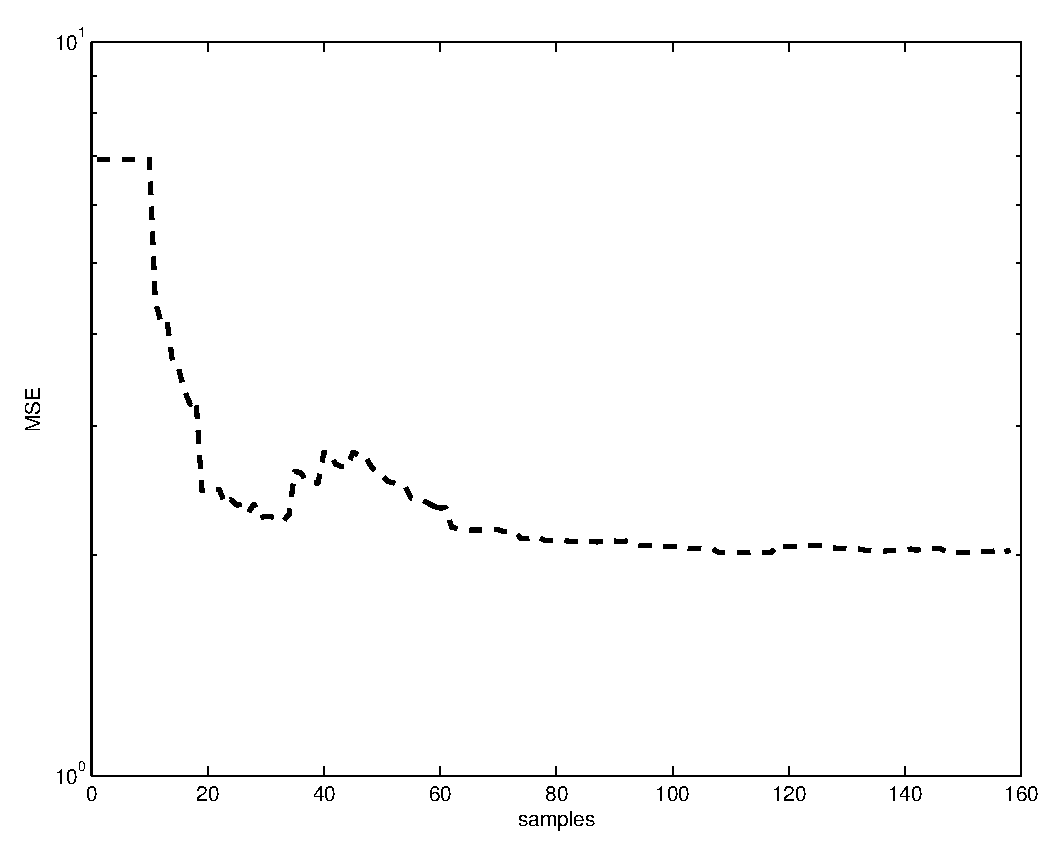
\includegraphics[width=4.0in, angle=0 ]{./Figure/jacobian-error.eps}
} \caption{Learning the arm jacobian. The plot represents the \emph{mse} on 
the test set during learning. See text.} 
\end{figure}
%



